%%%%%%%%%%%%%%%%%%%%%%%%%%% asme2ej.tex %%%%%%%%%%%%%%%%%%%%%%%%%%%%%%%
% Template for producing ASME-format journal articles using LaTeX    %
% Written by   Harry H. Cheng, Professor and Director                %
%              Integration Engineering Laboratory                    %
%              Department of Mechanical and Aeronautical Engineering %
%              University of California                              %
%              Davis, CA 95616                                       %
%              Tel: (530) 752-5020 (office)                          %
%                   (530) 752-1028 (lab)                             %
%              Fax: (530) 752-4158                                   %
%              Email: hhcheng@ucdavis.edu                            %
%              WWW:   http://iel.ucdavis.edu/people/cheng.html       %
%              May 7, 1994                                           %
% Modified: February 16, 2001 by Harry H. Cheng                      %
% Modified: January  01, 2003 by Geoffrey R. Shiflett                %
% Use at your own risk, send complaints to /dev/null                 %
%%%%%%%%%%%%%%%%%%%%%%%%%%%%%%%%%%%%%%%%%%%%%%%%%%%%%%%%%%%%%%%%%%%%%%

%%% use twocolumn and 10pt options with the asme2ej format
\documentclass[twocolumn,10pt]{asme2ej}
\usepackage{graphicx}
%\usepackage{auto-pst-pdf}
%\usepackage{epsfig} %% for loading postscript figures

%% The class has several options
%  onecolumn/twocolumn - format for one or two columns per page
%  10pt/11pt/12pt - use 10, 11, or 12 point font
%  oneside/twoside - format for oneside/twosided printing
%  final/draft - format for final/draft copy
%  cleanfoot - take out copyright info in footer leave page number
%  cleanhead - take out the conference banner on the title page
%  titlepage/notitlepage - put in titlepage or leave out titlepage
%  
%% The default is oneside, onecolumn, 10pt, final


\title{How many people are at intersections in Boston?}

%%% first author
\author{Ben Lawson
    \affiliation{
	Department of Computer Science\\
	Boston University\\
	Boston, Massachusetts 02215\\
        balawson@bu.edu 
    }	
}
\begin{document}

\maketitle    

%%%%%%%%%%%%%%%%%%%%%%%%%%%%%%%%%%%%%%%%%%%%%%%%%%%%%%%%%%%%%%%%%%%%%%
\begin{abstract}
{\it Social media is a constant factor in many people's lives in current times. We explore the usefulness of data collected from public resources to derive estimates of a subsection of people at different intersections in Boston. Using mainly Twitter data, we are able to apply sampling methods to determine an estimate of the monthly visitation rate of almost 60 intersections. This information can be incorporated into other systems to improve traffic congestion estimation.
}
\end{abstract}

%%%%%%%%%%%%%%%%%%%%%%%%%%%%%%%%%%%%%%%%%%%%%%%%%%%%%%%%%%%%%%%%%%%%%%

%%%%%%%%%%%%%%%%%%%%%%%%%%%%%%%%%%%%%%%%%%%%%%%%%%%%%%%%%%%%%%%%%%%%%%
\section{Introduction}

In this project, we attempt to develop an understanding of human movement within the city of Boston. Using social media data from three companies, Brightkite and Gowalla, both of which are no longer active, and Twitter. To generate higher granular information, we used OpenStreetMap data to associate social media user's posts to specific intersections. Since not all people use social media, and thus are not represented in the datasets presented here, we must infer the actual amount of people that are present at these intersections in real life. Future work will attempt to cross-validate these methods with different types of observations, such as census population data and population counts at intersections derived from street cams and computer vision. Future work will also include using this data to solve classic problems, like max flow, in the pedestrian setting. 

%%%%%%%%%%%%%%%%%%%%%%%%%%%%%%%%%%%%%%%%%%%%%%%%%%%%%%%%%%%%%%%%%%%%%%
\section{Data Resources}

Many types of data were used in this project. Three sources of geosocial media data were used as well as geographical information from OpenStreetMap
%%%%%%%%%%%%%%%%%%%%%%%%%%%%%%%%%%%%%%%%%%%%%%%%%%%%%%%%%%%%%%%%%%%%%%
\subsection{Brightkite Dataset}

This is a social media networking service that was acquired by a mobile social network, Limbo, in 2009. The dataset contains posts with a user id, geocoordinates, and a timestamp between 14 April 2008 and 18 October 2010.
%%%%%%%%%%%%%%%%%%%%%%%%%%%%%%%%%%%%%%%%%%%%%%%%%%%%%%%%%%%%%%%%%%%%%%
\subsubsection{Gowalla Dataset}
This is a social media networking service that went out of business. Each post in the dataset has a user id, geocoordinates, and a timestamp, dating between 23 April 2009 and 22 October 2010.


%%%%%%%%%%%%%%%%%%%%%%%%%%%%%%%%%%%%%%%%%%%%%%%%%%%%%%%%%%%%%%%%%%%%%%
\subsubsection{Twitter Dataset}
This is a micro blogging service that collects geological information about users's posts. This is still an active service and this data set was collected from 11 May 2015 until 2 April 2016. This data was collected via Twitter's streaming API, filtered by geolocation.

%%%%%%%%%%%%%%%%%%%%%%%%%%%%%%%%%%%%%%%%%%%%%%%%%%%%%%%%%%%%%%%%%%%%%%
%%%%%%%%%%%%%%%% begin figure %%%%%%%%%%%%%%%%%%%
%%% 3.34in is the maximum width you can have for a figure
\begin{figure} 
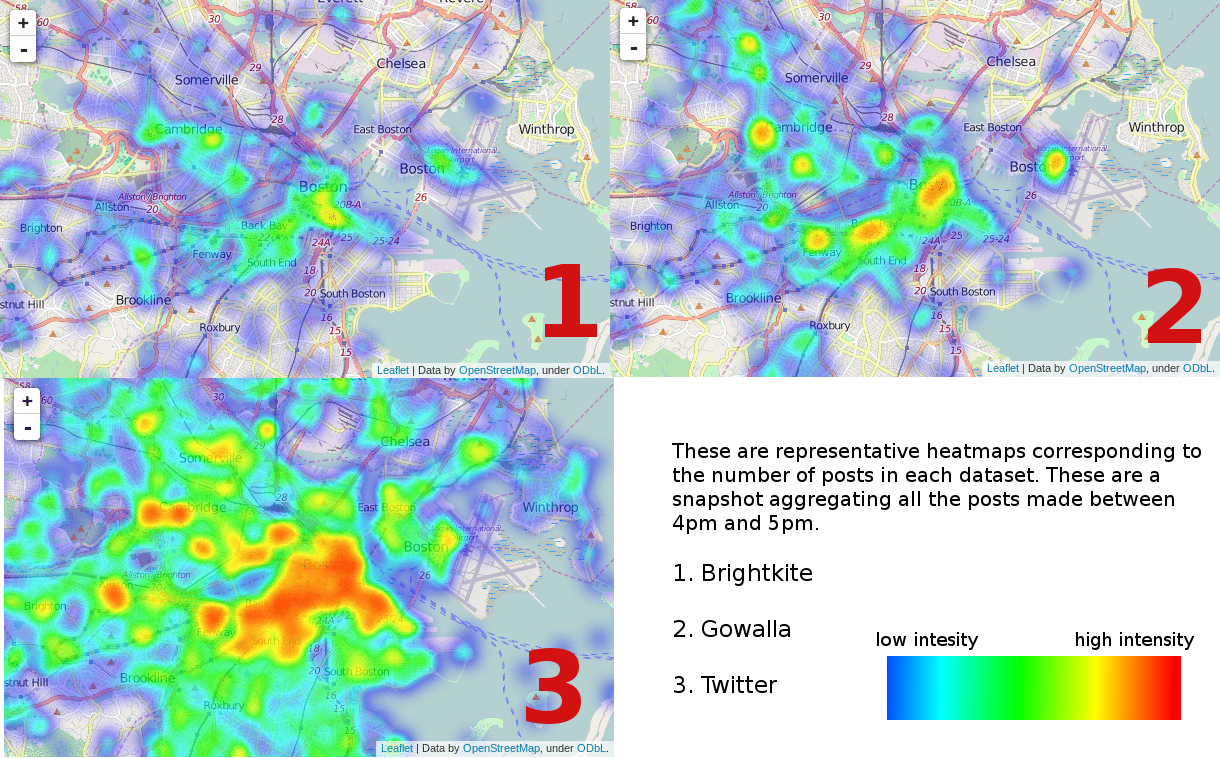
\includegraphics[scale=0.23]{heatmap.png}
\caption{Heatmap of tweets by direct count. Scaled proportionally total to each dataset.}
\end{figure}
%%%%%%%%%%%%%%%% end figure %%%%%%%%%%%%%%%%%%%
%%%%%%%%%%%%%%%% begin figure %%%%%%%%%%%%%%%%%%%
%%% 3.34in is the maximum width you can have for a figure
\begin{figure} 
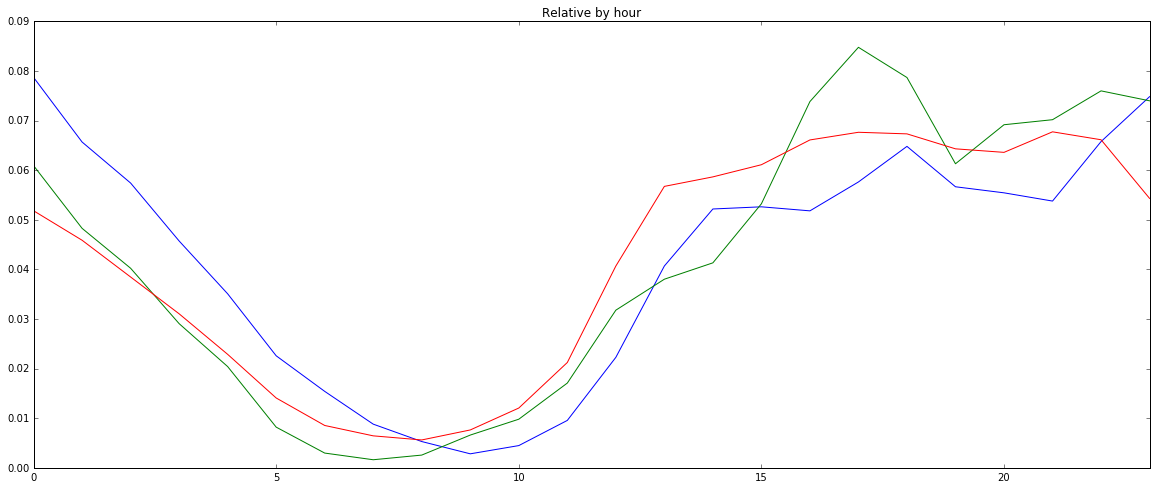
\includegraphics[scale=0.2]{postsbyhour.png}
\caption{Shows the percentage of tweets by hour. Demostrates that tweeting behavior mimics the human sleep cycle. Red is Brightkite, Green is Gowalla, and Blue is Twitter.}
\end{figure}
%%%%%%%%%%%%%%%% end figure %%%%%%%%%%%%%%%%%%%

\subsection{OpenStreetMap}

This dataset was collected from OpenSteetMap, a collaborative, community based geographical open data resource. We use the labeled roads in the Boston area to create a chart of intersections. 

\subsection{BostonMaps: Open Data}
This dataset contained bounding boxes and geometric shapes for each of the neighboorhoods in Boston. This was used to help give a general intuition for results.
\section{Segmentation}
Using the OpenStreetMap data, each Twitter post was associated with the closest intersection. This was done for each month in the Twitter dataset, so twelve months are represented from May 2015 to April 2016.
\section{Sampling}
\textit{Capture \& Recapture}. This type of sampling was first used when measuring animals in traps. Trappers would mark animals and then count how many of these animals returned to derive an estimate of the total population.
%%%%%%%%%%%%%%%% begin figure %%%%%%%%%%%%%%%%%%%
\begin{figure} 
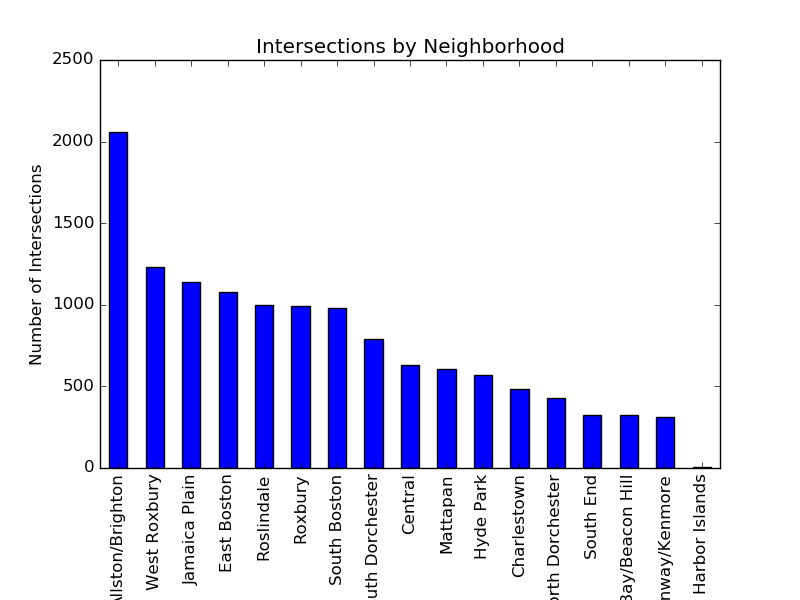
\includegraphics[scale=0.4]{numberofintersections.png}
\caption{The number of intersections per neighborhood}
\end{figure}
%%%%%%%%%%%%%%%% end figure %%%%%%%%%%%%%%%%%%%
%%%%%%%%%%%%%%%% begin figure %%%%%%%%%%%%%%%%%%%
\begin{figure} 
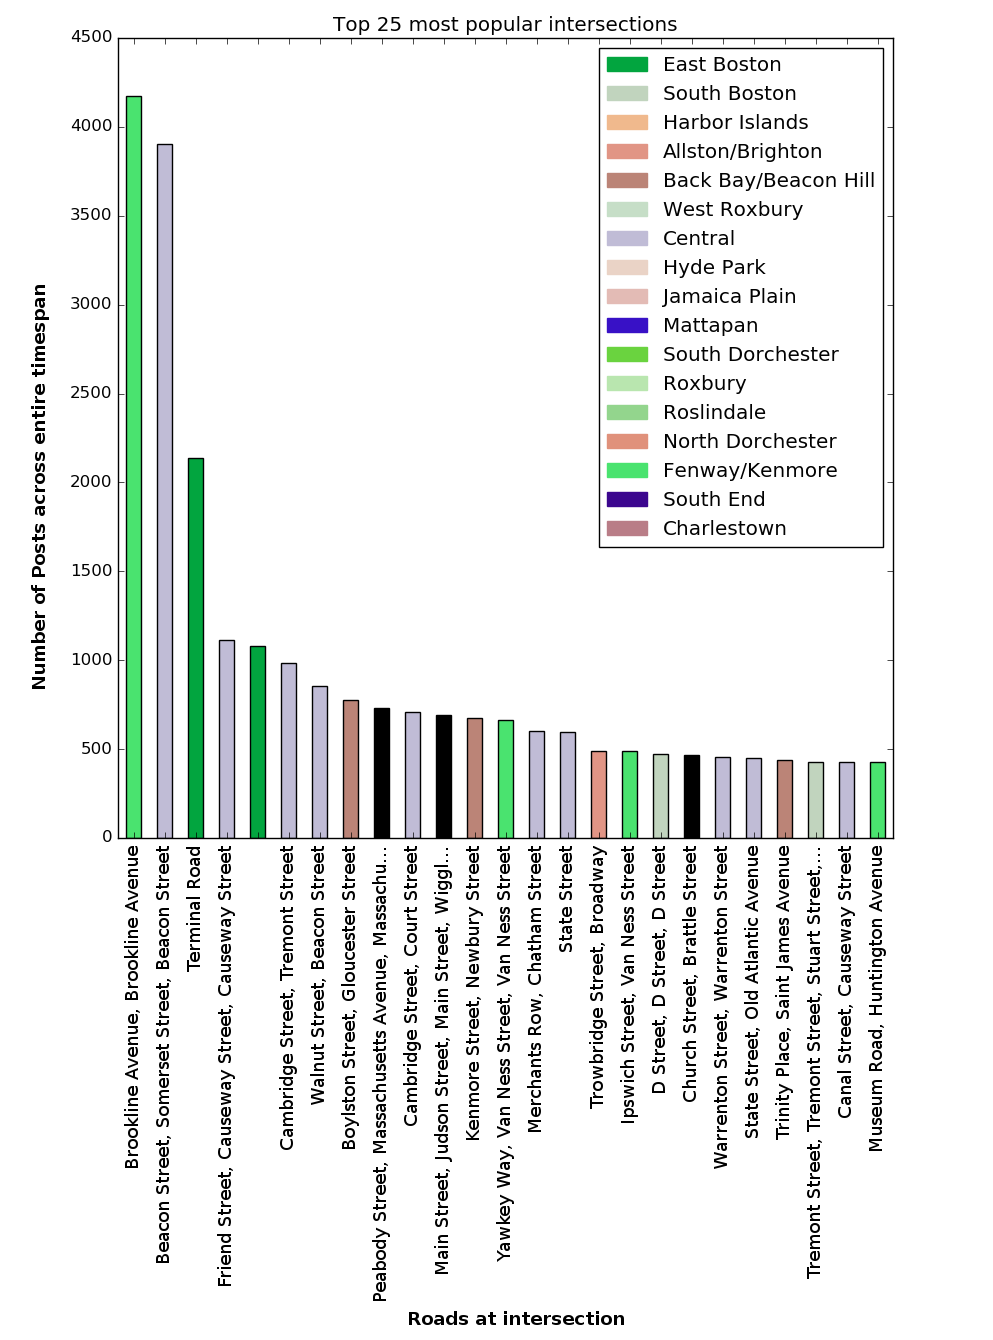
\includegraphics[scale=0.3]{popularintersections.png}
\caption{The 25 most popular intersections overall (sheer volumne) colored by neighboorhood. Note missing road names and black color is due to missing data.}
\end{figure}
%%%%%%%%%%%%%%%% end figure %%%%%%%%%%%%%%%%%%%
\begin{figure}
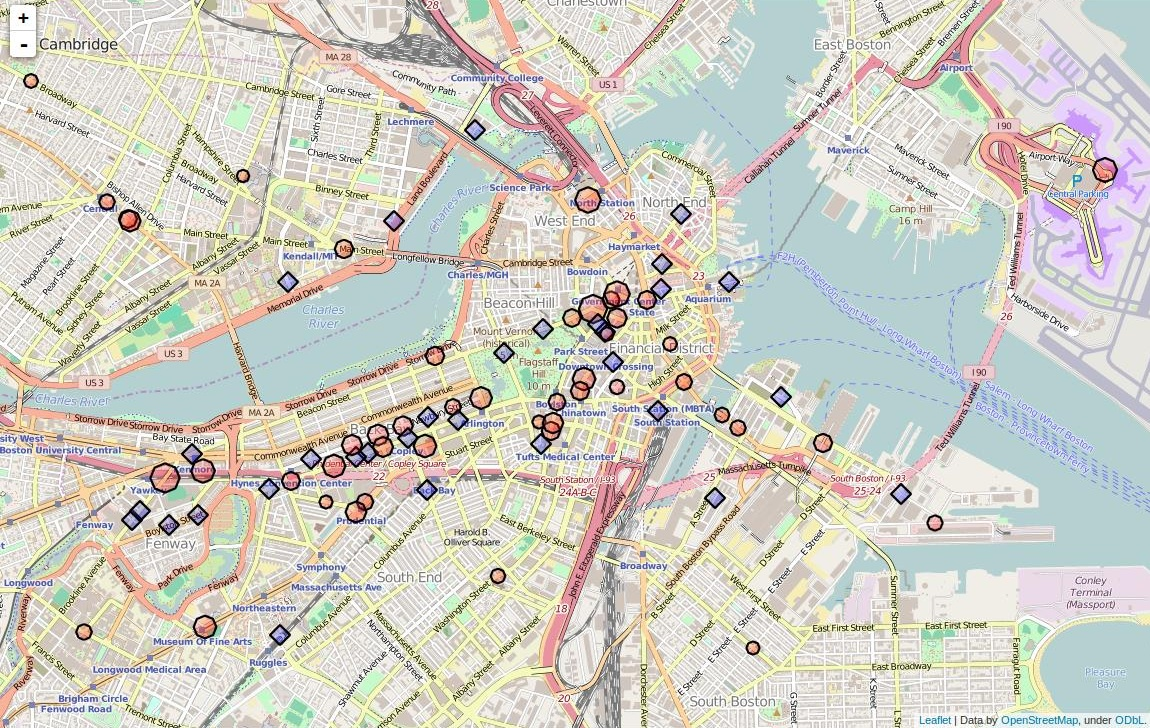
\includegraphics[scale=0.2]{estimate.jpg}
\caption{Relative estimates for monthly social media users per intersection}
\end{figure}
%%%%%%%%%%%%%%%% end figure %%%%%%%%%%%%%%%%%%%
We discovered only 94 intersections, of the almost 25,000, had five or more visitors each month. Only 57 of these intersections had visitors that returned during the capture/recapture period. The red markers show the intersections that estimates could be computed, scaled with the $\log_2$ function. The blue markers show the intersections that did not have returning users. Fenway park had that max estimate with approximately 12,000 visitors per month. This calculation was only done with the Twitter dataset. Future work will explore the best way to intergrate the Brightkite and Gowalla datasets.


\begin{equation}
\hat{N} = \frac{Kn}{k}
\end{equation} 

$\hat{N}$ is the estimation of the total population of social media users, $n$ is the number of users during the first month, $K$ is the number of users during the second month, and $k$ is the number of users from the first month that are observed during the second month. With this formulation, we can derive estimations for the number of social media users that post near an intersection per month. It will be important to discover what percentage the social media users are of the total population. This can be done by observing a true population through web cams and utilizing popular methods in computer vision, like object dectection and background subtraction. We can also obtain an estimate by comparing all the social media activity in a neighborhood to the total population take from the census, however this would be less accurate and would be difficult to argue as the true population.

\begin{equation}
\frac{| A \cap B|}{|B|} = \frac{|A \cap S|}{|S|} = \frac{|A|}{|S|}
\end{equation}
Once we know the relationship between the number of social media users and the true total population, we can use proportional sampling to determine the most accurate estimate for the number of people passing through an intersection. For example, if we knew that $\frac{1}{10}$ people used social media, we can use Equation(2) to determine the estimate of people at each intersection, instead of an estimate of the number of social media users at each intersection. If we take the most popular intersection, Brookline Ave @ Brookline Ave, our estimate is 12,835.2. Plugging this into the formula gives us: $\frac{1}{10} = \frac{12835.2}{\hat{N}}$ resulting in an appromation of $128,352$ total people passing through that intersection each month.

%%%%%%%%%%%%%%%%%%%%%%%%%%%%%%%%%%%%%%%%%%%%%%%%%%%%%%%%%%%%%%%%%%%%%%
\section{Conclusions}
Although the social media data consisted of many posts, only a fraction of the intersections had data spanning the entire collection period. Of these intersections, only a fraction had entire data to compete the estimate via the capture \& recapture method. Future work will be to include the Brightkite and Gowalla datasets in the estimation of intersection occupancy and analyzing flow problems associated with pedestrian traffic.

%%%%%%%%%%%%%%%%%%%%%%%%%%%%%%%%%%%%%%%%%%%%%%%%%%%%%%%%%%%%%%%%%%%%%%
%%%%%%%%%%%%%%%%%%%%%%%%%%%%%%%%%%%%%%%%%%%%%%%%%%%%%%%%%%%%%%%%%%%%%%
\begin{acknowledgment}
Special thanks to Andrei Lapets who supported this project and helped flush out ideas about general project direction. Special thanks to Evimaria Terzi for help with the development of the Twitter dataset and Sofia Maria Nikolakaki for her work with tweet segmentation by intersection.
\end{acknowledgment}

\section*{Appendix A: Most Popular Intersections (monthly estimates)}
\begin{tabular}{| l | r |}
\hline
Road Intersection & Monthly Estimate \\
\hline
\hline
Brookline Ave, Brookline Ave & 12835.2 \\
\hline
Beacon St, Somerset St & 9226.3\\
\hline
Friend St, Causeway St & 3685.0 \\
\hline
Cambridge St, Court St & 3596.0 \\
\hline
Main St, Judson St, Wigglesworth St & 2928.0 \\
\hline
Terminal Road & 2135.2 \\
\hline
Kenmore St, Newbury St & 1840.0 \\
\hline
Avenue De Lafayette, Washington St & 1392.0 \\
\hline
Trinity Place, Saint James Avenue & 1368.0 \\
\hline
Boylston St, Gloucester St & 1357.3 \\
\hline
Museum Road, Huntington Avenue & 1323.0 \\
\hline
Arlington St, Newbury St & 1020.0 \\
\hline
Massachusetts Ave, Douglass St & 783.0 \\
\hline
Newbury St, Exeter St & 726.0 \\
\hline
Belvidere St, Huntington Ave & 704.0 \\
\hline
Tremont St, Stuart St & 640.0 \\
\hline
Fairfield St, Newbury St & 580.0 \\
\hline
Boylston St, Exeter St & 528.0 \\
\hline
Dartmouth St, Newbury St & 455.0 \\
\hline
School St, Province St & 448.0 \\
\hline
Church St, Brattle St & 387.8 \\
\hline
Tremont St, Seaver Place & 320.0 \\
\hline
Back St, Berkeley St & 320.0 \\
\hline
Washington St, Hayward Place & 312.0 \\
\hline
Main St & 310.5 \\
\hline
World Trade Center Road & 300.0 \\
\hline
State St, Congress St & 286.0 \\
\hline
Cambria St, Boylston St & 270.0 \\
\hline
Massachusetts Ave, Brookline St & 250.8 \\
\hline
Park St, Beacon St & 250.0 \\
\hline
Brattle St, Massachusetts Ave, JFK St & 243.8 \\
\hline
Chester St, Elm St & 238.0 \\
\hline
Wadsworth St, Madison St & 237.6 \\
\hline
Cambridge St, Tremont St & 203.1 \\
\hline
Boylston St, Tremont St & 180.9 \\
\hline
Huntington Avenue & 156.0 \\
\hline
Atlantic Avenue, Congress St & 135.0 \\
\hline
Berkeley St, Newbury St & 130.0 \\
\hline
Massachusetts Ave, Essex St & 116.0 \\
\hline
Blackfan St, Longwood Ave & 115.0 \\
\hline
Farnsworth St, Congress St & 114.0 \\
\hline
Drydock Ave, Tide St & 102.0 \\
\hline
Congress St & 91.0 \\
\hline
Bedford St, Kingston St & 84.0 \\
\hline
Washington St, Union Park St & 80.0 \\
\hline
Highland Ave, Central St & 78.0 \\
\hline
Franklin St, Pearl St & 65.0 \\
\hline
Ellery St, Broadway & 64.0 \\
\hline
Florence St, Louise Road & 57.8 \\
\hline
Province St, Bromfield St & 56.0 \\
\hline
Stuart St, Warrenton St & 52.5 \\
\hline
\end{tabular}
\end{document}
